
\documentclass{article}
\usepackage{arxiv}
\usepackage[utf8]{inputenc} % allow utf-8 input
\usepackage[T1]{fontenc}    % use 8-bit T1 fonts
\usepackage{hyperref}       % hyperlinks
\usepackage{url}            % simple URL typesetting
\usepackage{booktabs}       % professional-quality tables
\usepackage{amsfonts}       % blackboard math symbols
\usepackage{nicefrac}       % compact symbols for 1/2, etc.
\usepackage{microtype}      % microtypography
\usepackage{lipsum}
\usepackage[]{algorithm2e}
\usepackage{graphicx}
\usepackage{enumitem}




\title{Hierarchical Leader Election Algorithm with remoteness constraint}


\author{
  P.~Kuznetsov \\
  INFRES Department\\
  Télécom ParisTech\\
  Paris, France \\
  \texttt{petr.kuznetsov@telecom-paristech.fr} \\
  \And
  A.~Diaconescu \\
  INFRES Department\\
  Télécom ParisTech\\
  Paris, France \\
  \texttt{ada.diaconescu@telecom-paristech.fr} \\
  \And
  M.~Tbarka \\
  Department of Software Engineering\\
  ENSIAS\\
  Rabat, Maroc \\
  \texttt{mohamed.tbarka@telecom-paristech.fr} \\
  %% \AND
  %% Coauthor \\
  %% Affiliation \\
  %% Address \\
  %% \texttt{email} \\
  %% \And
  %% Coauthor \\
  %% Affiliation \\
  %% Address \\
  %% \texttt{email} \\
  %% \And
  %% Coauthor \\
  %% Affiliation \\
  %% Address \\
  %% \texttt{email} \\
}

\begin{document}
\maketitle

\begin{abstract}
A hierarchical algorithm for electing a leaders' hierarchy in an asynchronous network with dynamically changing communication topology is presented including a remoteness's constraint towards each leader. The algorithm ensures that, no matter what pattern of topology changes occur, if topology changes cease, then eventually every connected component contains a unique leaders' hierarchy. The algorithm combines ideas from the Temporally Ordered Routing Algorithm (TORA) for mobile ad hoc networks with a wave algorithm, all within the framework of a height-based mechanism for reversing the logical direction of communication links. Moreover, an improvement from the algorithm in is the introduction of logical clocks as the nodes’ measure of time, instead of requiring them to have access to a common global time. This new feature makes the algorithm much more flexible and applicable to real situations, while still providing a correctness proof. It is also proved that in certain well behaved situations, a new leader is not elected unnecessarily.
\end{abstract}


% keywords can be removed
\keywords{leader election \and hierarchical algorithm}

\section{Preliminaries}

\subsection{System Model}
We assume a system consisting of a set $P$ of computing nodes and a set $L$ of bidirectional communication links between nodes. $L$ consists of one link for each unordered pair of nodes, i.e., every possible link is represented. The nodes are assumed to be completely reliable. The links between nodes go up and down, due to the movement of the nodes. While a link is up, the communication across it is in first-in-first-out order and is reliable but asynchronous.

We model the whole system as a set of (infinite) state machines that interact through shared events (a specialization of the IOA model \cite{kour2014real}). Each node and each link is modeled as a separate state machine. The shared events are Link Up/Down notifications and receipt of messages, all of which are controlled and initiated by the link and responded to by the node. The sending of a message is also a shared event, but it is controlled and initiated by the node and responded to by the link; we are not explicitly modeling this.

The next subsection gives more details about how links are modeled and specifies the initial states. The algorithm executed by the nodes and its initial states are described in Section 3.
\subsection{Modeling Asynchronous Dynamic Links}
We now specify how communication is assumed to occur over the dynamic links, and how notification of a link’s status is synchronized at the two endpoints of the link.

The state of a link $Link_{u, v}$, which models the bidirectional communication link between node u and node v, consists of a status variable and two queues of messages.

The possible values of the status variable are $Up$, $GoingDown_{u}$ , $GoingDown_{v}$, $Down$, $ComingUp_{u}$, and $ComingUp_{v}$. The link transitions among different values of its status variable through $LinkUp$ and $LinkDown$ events. Figure 1 shows the state transition diagram for $Link_{u, v}$. The intuition is that if a $LinkUp$ (resp., $LinkDown$) occurs at one endpoint of the link, then $LinkUp$ (resp., $LinkDown$) must occur at the other endpoint before $LinkDown$ (resp., $LinkUp$) can occur at either end.

The other components of the link’s local state are the two message queues: $mqueue_{u,v}$ holds messages in transit from $u$ to $v$ and $mqueue_{v,u}$ holds messages in transit from $v$ to $u$.

An attempt by node $u$ to send a message to node $v$ results in the message being appended to $mqueue_{u,v}$ if the link’s status is either $ComingUp_u$ or $Up$; otherwise there is no effect.

\begin{figure}[hbtp]
\centering
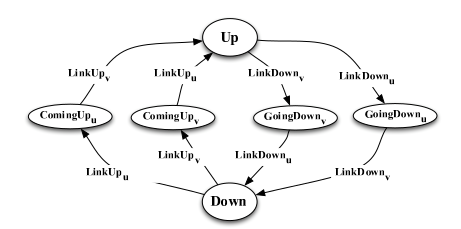
\includegraphics[scale=.75]{screenshot.png}
\caption{State diagram for status variable of $Link_{u, v}$.}
\end{figure}

If the status is $ComingUp_u$ , then messages in transit from $u$ to $v$ are held in the queue until $v$ has been notified that the link is $Up$. Once the link is $Up$, the event by which node $u$ receives the message at the head of $mqueue_{v,u}$ is enabled to occur. An attempt by node $v$ to send a message to node $u$ is handled analogously.

Whenever a $LinkDown_u$ or $LinkDown_v$ event occurs, both message queues are emptied. Neither $u$ nor $v$ is alerted to which messages in transit have been lost due to the $LinkDown$.

In an initial state of the link, both message queues are empty and the status is either $Up$ or $Down$.

\subsection{Configurations and Executions}
The notion of configuration is used to capture an instantaneous snapshot of the state of the entire system. A configuration is a vector of node states, one for each node in $P$, and a vector of link states, one for each link in $L$.
Assume that the undirected graph $G = (V, E)$ defines the initial communication topology of the system, where $V$ is a set of vertices corresponding to the set $P$ of nodes, and E is a set of edges corresponding to the set of communication links that are up. In an initial configuration with respect to $G$, each node is in an initial state (as prescribed by the node’s algorithm), each link corresponding to an edge in $E$ is in an initial state with its status equal to Up, and every other link has its status equal to Down.
Define an execution as an infinite sequence $C_0, e_1 ,C_1, e_2 ,C_2, ...$ of alternating configurations and events, starting with an initial configuration and, if finite, ending with a configuration, that satisfies the following safety conditions:
\begin{itemize}
\item $C_0$ is an initial configuration (w.r.t. some initial topology $G$).
\item The preconditions for event are true in $C_{i-1}$ for all $i\geq 1$.
\item $C_i$ is the result of executing event $e_i$ on configuration $C_{i - 1}$ , for all $i \geq 1$ (only the node and link involved in an event change state, and they change according to their state machine transitions).
\end{itemize}

An execution also satisfies the following liveness conditions:
\begin{itemize}
\item If a link remains Up for infinitely long, then every message sent over the link is eventually delivered.
\item For each link, if only a finite number of link events occur, then the link status after the last one is either Up or Down (not in between).
\end{itemize}

We also assign a positive real-valued global time gt to each event $e_i$, $i ≥ 1$, such that $gt(e_i) < gt(e_{i + 1}^)$ and, if the execution is infinite, the global times increase without bound. Each configuration inherits the global time of its preceding event, so $gt(C_i) = gt(e_i)$ for $i \geq 1$; we define $gt(C_0)$ to be $0$. We assume that the nodes do not have access to $gt$.

\subsection{Problem Definition}
Each node u in the system has a local variable $lid_{u}$ to hold the identifier of the node currently considered by u to be the supreme leaders o the connected component containing u, and another local variable $slid_u$ to hold the identifier of the node currently considered by u to be the sub-leader in such a way that the distance to this subèleader does not exceed a certain constant d (the remoteness constraint). The set of all the leaders including the supreme one forms a spanning tree as subgraph of the DAG established.
In every execution that includes a finite number of topology changes, we require that the following eventually holds:
\begin{itemize}
\item Every connected component $CC$ of the final topology contains a node $l$, the supreme leader, such that $l$ is the only node which verifies $ lid_{l} = l $.
\item For each node u of each component $CC$, different from the supreme leader, a node v exists such as $slid_{u} = v$ and $d_{u,v} < D$ ($D$ is the maximum remoteness towards a leader and the $ d_{u,v} $ is the shortest distance between $u$ and $v$)
\end{itemize}

In a more formal way, one can state the problem as follows:\\
In every execution that includes a finite number of topology changes, we require that the following eventually holds:

\begin{itemize}
\item For each node $ u $ of every connected component $CC$ of the final topology:
$u$ selects $(slid_u, pre_u)$, ${(slid_u, pre_u) \in N_u \times N_u}$ such that ${(slid_u, pred_u)}_{u \in CC}$ is a spanning tree $T$ ($slid_u$ (resp. $pred_u$) is the sub-leader (resp. the predecessor to reach $lid_u$) considered as such by i.
\item For each node $u$, different from the root of $T$, of every connected component $CC$ of the final topology:\\
if $ (k-1)D < depth_T (i) <= kD, k \in IN $, then $ depth_T(lid_i)=(k-1)D$ ($depth_T(u)$ is the depth of u in T)
\end{itemize}



Our algorithm also ensures that eventually each link in the system has a direction imposed on it by virtue of the data stored at each endpoint such that each connected component CC is a leader-oriented DAG containing a spanning tree, i.e., every node has a directed path to its local leader respecting, among the other leaders, a certain hierarchy containing one supreme leader.

\newpage
\section{Hierarchical Leader Election Algorithm}
In this section, we present our hierarchical leader election algorithm. The pseudocode for the algorithm is presented in Figures 1, 2 and 3. First, we provide an informal description of the algorithm, then, we present the details of the algorithm and the pseudocode, and finally, we provide an example execution. In the rest of this section, variable $var$ of node $u$ will be indicated as $var_u$. For brevity, in the pseudocode for node $u$, variable $var_u$ is denoted by just $var$^.

\subsection{Informal Description}
Each node in the system has a 7-tuple of integers called a height. The directions of the edges in the graph are determined by comparing the heights of neighboring nodes:
an edge is directed from a node with a larger height to a node with a smaller height.
Due to topology changes nodes may lose some of their incident links, or get new ones
throughout the execution. Whenever a node loses its last outgoing link because of a
topology change, it has no path to the current leader, so it reverses all of its incident
edges. Reversing all incident edges acts as the start of a search mechanism (called
a reference level) for the current leader. Each node that receives the newly started
reference level reverses the edges to some of its neighbors and in effect propagates
the search throughout the connected component. Once a node becomes a sink and
all of its neighbors are already participating in the same search, it means that the
search has hit a dead end and the current leader is not present in this part of the
connected component. Such dead-end information is then propagated back towards
the originator of the search. When a node which started a search receives such dead-
end messages from all of its neighbors, it concludes that the current leader is not
present in the connected component, and so the originator of the search elects itself
as the new leader. Finally, this new leader information propagates throughout the
network via an extra “wave” of propagation of messages. The same "wave" will establish the hierarchy of leaders by comparing, each time, the $\delta$ (distance) of each neighbor of the current node; if this danstance is different than a multiple of the maximum or zero, the node adopts the leader of this neighbor, otherwise, it adopts it, the concerned neighbor, as a leader. This "wave" assures the aspect of hierarchy in our algorithm.

In our algorithm, two of the components of a node’s height are timestamps recording the time when a new “search” for the leader is started, and the time when a leader is elected. In the algorithm in [15], these timestamps are obtained from a global clock accessible to all nodes in the system. In this paper, we use the notion of causal clocks instead.

One difficulty that arises in solving leader election in dynamic networks is dealing
with the partitioning and merging of connected components. For example, when a
connected component is partitioned from the current leader due to links going down,
the above algorithm ensures that a new leader is elected using the mechanism of
waves searching for the leader and convergecasting back to the originator. On the
other hand, it is also possible that two connected components merge together resulting
in two leaders in the new connected component. When the different heights of the two
leaders are being propagated in the new connected component, eventually, some node
needs to compare both and decide which one to adopt and continue propagating.
Recall that when a new leader is elected, a component of the height of the leader
records the time of the election which can be used to determine the more recent
of two elections. Therefore, when a node receives a height with a different leader
information from its own, it adopts the one corresponding to the more recent election.

Similarly, if two reference levels are being propagated in the same connected
component, whenever a node receives a height with a reference level different from
its current one, it adopts the reference level with the more recent timestamp and con-
tinues propagating it. Therefore, even though conflicting information may be prop-
agating in the same connected component, eventually the algorithm ensures that as
long as topology changes stop, each connected component has a unique leader.

\subsection{System Model}
In this section, we explain the local variables used in our leader election algorithm. The pseudocode for the algorithm is presented in Figures 3.1, 3.2 and 3.3. An overview and sample execution is given in Section 3.1. In the analysis, variable v of node i will be indicated as v i.

Each node i keeps an array of heights, height i , with an entry for itself and for each of its neighbors, in which it stores the most recent height information that it has received for those nodes.

Each height is a 7-tuple, with the following components:
\begin{enumerate}
\item τ , a nonnegative timestamp that is either 0 or the time when the current search for an alternate path to the leader was initiated
\item oid, a nonnegative value that is either 0 or the id of the node that started the current search
\item r, a bit that is set to 0 when the current search is initiated and set to 1 when the current search hits a deadend
\item δ , an integer that is set to ensure that links are directed appropriately to neighbors with the same first three components
\item nlts, a nonpositive timestamp whose absolute value is the time when the current leader was elected
\item lid, the id of the current leader
\item id, the id of the node
\end{enumerate}
Components ( τ , oid, r) are referred to as the reference
level, or RL; ( τ , oid) alone are referred to as the reference
level prefix; and (nlts, lid) is referred to as the leader pair
or LP. The components of entry k in height i are referred to
as ( τ k , oid k , r k , δ k , nlts k , lid k , k) in the pseudocode.

Nodes communicate over links during the algorithm ex-
ecution by sending Update messages. Each message con-
tains the height tuple and the logical clock timestamp of the
sending node. The link between node i and one of its neigh-
boring nodes j is considered by i to be outgoing (directed
from i to j) if and only if height i [i] > height i [ j]. That is,
node i uses the information in its local state concerning it-
self and node j to determine (its view of) the direction of the
link to j. Because of message delays, it is not necessarily
the case that i and j have consistent views of the direction
of the link between them.

Other events that occur at a node are formations
(LinkUps) and failures (LinkDowns) of links. Suppose the
most recent indication that node i has received concerning
the link between itself and node j is a LinkUp. If i has re-
ceived a message from j since that LinkUp, then i considers
j as one of its neighbors, and stores the id of j in its local
variable N i . If i has not yet received a message from j, then
the link is considered as still forming, and i stores the id of j
in its local variable forming i ; j is not considered a neighbor
of i (yet).

Nodes have no access to global time, but, instead, each
of them has a local logical clock [11]. A logical clock is
a non-negative integer, initially 0. Logical clocks can be
updated in two possible ways, depending on the type of the
event occurring at a node. If a LinkUp or a LinkDown event
occurs at a node, its logical clock is incremented by 1. Oth-
erwise, if a node receives an Update message, the logical
clock is set to one more than the maximum of the node’s
current logical clock value and the timestamp included in
the message. This way, we ensure that for each node, the
value of its logical clock is non-decreasing for each subse-
quent event. The logical clock of a node is referred to as LC
in the pseudocode.

Given an initial connected communication graph G =
(V, E), with V corresponding to the set of nodes and E to
the set of communication links that are up, the initial state
of each node i is defined as follows 1 .
\begin{enumerate}
\item forming i is empty
\item N i contains the id of every node j such that the vertices
in V corresponding to i and j are neighbors in G
\item height i [i] = (0, 0, 0, δ i , 0, l, i), where l is the id of a
fixed node in i’s connected component, the current
leader
\item for each neighbor j of i, height i [ j] = height j [ j] (i.e., i
has accurate information about j’s height)
\item LC i = 0 (i.e. the logical clocks of all nodes are initially
set to 0).
\end{enumerate}
Furthermore, for each node i, δ i equals the distance from i
to l; this condition ensures that every node has a directed
path to l.
Next we define the conditions under which a node con-
siders itself to be a sink.
\begin{itemize}
\item SINK = ((LP i j = LP ii ∀ j ∈ N i ) and (height i [i] <
min{height i [ j] ∀ j ∈ N i }) and (lid ii , i)). This pred-
icate is true when, according to i’s local state, i is not
a leader, has all neighbors with the same LP, and has
no outgoing links. If node i has links to any neighbors
with different LPs, i is not considered a sink, regard-
less of the directions of those links.
\end{itemize}
\subsection{Overview of Algorithm}
We depict the network as a DAG in which each bidirec-
tional communication link points from a node with lexico-
graphically higher height to another node with lexicograph-
ically lower height. Nodes send algorithm messages only
when they change the contents of their height tuple. The
contents of the height tuple at a particular node are changed
only when the node elects itself a leader, when it changes its
current leader, or when it loses its last outgoing link to its
current leader. The network is quiescent when there is no
message in transit on any link. Messages that do not cause
a node to lose its last outgoing link to its current leader or
to change its current leader result only in a change to the
internal data that node keeps about its neighbors’ heights.
Figure 3.4 shows a sample execution of the algorithm.
Each part (a)–(h) is discussed below.
\begin{enumerate}[label=\alph *)]
\item A quiescent network is a leader-oriented DAG in
which node H is the current leader. The height of each
node is displayed in parenthesis. Link direction in this
figure is shown using solid-headed arrows and mes-
sages in transit are arrows with outlined heads super-
imposed on the links that point from message sender
to receiver.
\item When non-leader node G loses its last outgoing link
due to the loss of the link to node H, G increments
its logical clock by 1, executes subroutine START -
N EW R EF L EVEL and takes on RL (1,G,0) and δ = 0.
Then node G sends messages with its new height to all
its neighbors. By raising its height in this way, G has
started a search for leader H.
\item Nodes D, E, and F receive the messages sent from node
G, messages that cause each of these nodes to take on
RL (1,G,0), set its δ to −1, ensuring that its height is
lower than G’s but higher than the other neighbors’.
Moreover, each of these nodes also updates its logical
clock to 2. Then D, E and F send messages to their
neighbors.
\item Node B has received messages from both E and D with
the new RL (1,G,0), and C has received a message
from F with RL (1,G,0); as a result, B and C take on
RL (1,G,0) with δ set to −2, update their logical clocks
to 3 and send messages. Additionally, as a result of the
messages sent by D, E, and F, node G updates its logi-
cal clock to 3.
\item Node A has received message from both nodes B and
C. In this situation, node A is connected only to nodes
that are participating in the search started by node G
for leader H. In this case, node A “reflects” the search
by setting the reflection bit in the (1,G,*) reference
level to 1, resetting its δ to 0, and sending its new
height to its neighbors. Moreover, nodes A, D, E, and
F update their clocks to 4.
\item Nodes B and C take on the reflected reference level
(1,G,1) and set their δ to −1, causing their heights to
be lower than A’s and higher than their other neigh-
bors’. They also update their logical clocks to 5 and
send their new heights to their neighbors.
\item Nodes D, E, and F act similarly as B and C did in part
(f), but set their δ variables to −2. As a result from
the messages sent by B and C, nodes A, D, E, and F
update their logical clocks to 6.
\item When node G receives the reflected reference level
from all its neighbors, it knows that its search for H is
in vain. G updates its logical clock to 7 and then elects
itself. The new LP (-7,G) then propagates through the
component, updating nodes’ logical clocks along the
way, assuming no further link changes occur; eventu-
ally each node has RL (0,0,0) and LP (-7,G), with D,
E and F having δ = 1, B and C having δ = 2, and A
having δ = 3.
\end{enumerate}
\newpage
\begin{figure}[hbtp]
\centering
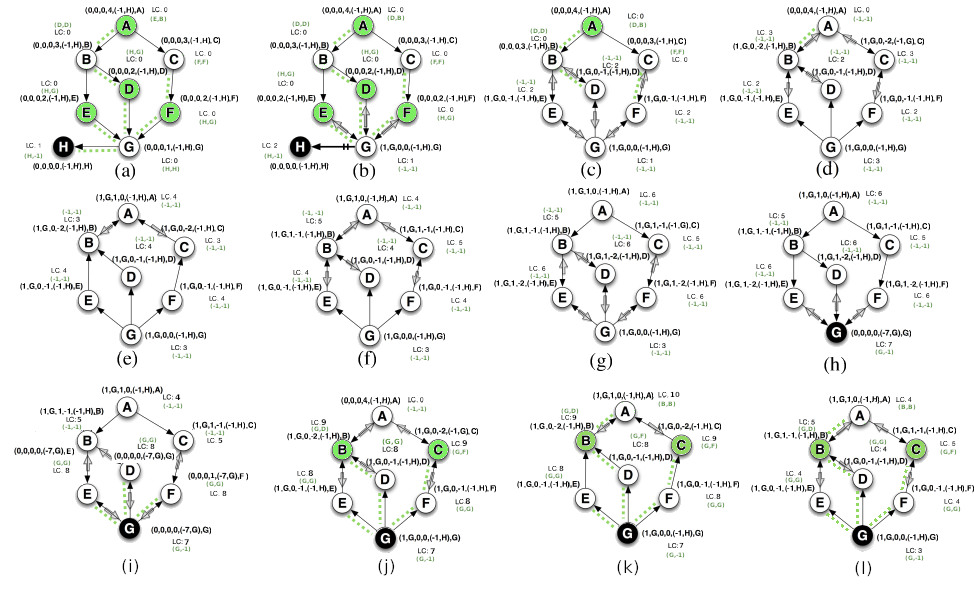
\includegraphics[scale=.5]{sample_execution.png}
\caption{Simple execution when leader H becomes disconnected (a), with time increasing from (a)–
(h). With no other link changes, every node in the connected component will eventually adopt G as
its leader}
\end{figure}

\newpage
\begin{figure}[hbtp]
\textbf{When $ChannelDown_{uv}$ event occurs}

\begin{enumerate}
\item \quad $ N := N\backslash \left\lbrace v\right\rbrace $
\item \quad $ forming := forming \backslash \left\lbrace v\right\rbrace $
\item \quad \textbf{if} $ (N = \emptyset )$
\item \quad \quad $ELECTSELF$
\item \quad \quad send Update($heigth[u]$) to all $ w\in forming$
\item \quad \textbf{else if}(SINK)
\item \quad \quad $STARTNEWREFLEVEL$
\item \quad \quad send Update($heigth[u]$) to all $w\in (N \cup forming)$
\item \quad \textbf{else if} $(j=pred_i)$
\item \quad \quad $pred_i=min \left\lbrace k \quad \vert \quad k\in N_i \quad and \quad \delta_k = \delta_j \right\rbrace$
\item \quad \textbf{end if}
\end{enumerate}


\textbf{When $ChannelUp_{uv}$ event occurs}

\begin{enumerate}
\item \quad $forming := forming \cup {v}$
\item \quad send Update($height[u]$) to all $ w \in (N \cup forming)$
\end{enumerate}
\caption{Code triggered by link change}
\end{figure}

\begin{figure}[hbtp]

\textbf{ELECTSELF}
\begin{enumerate}
\item $ height[i] := (0,0,0,0,-LC_{i},i,i) $
\end{enumerate}

\textbf{REFLECTREFLEVEL}
\begin{enumerate}
\item $ height[i] := (\tau ,oid,1,0,nlts^{i},lid^i,i) $
\end{enumerate}


\textbf {REFLECTREFLEVEL}
\begin{enumerate}
\item $ height[i] := (\tau ,oid,1,0,nlts^{i},lid^i,i) $
\end{enumerate}


\textbf{PROPAGATELARGESTREFLEVEL}
\begin{enumerate}
\item $ (\tau , oid^{i}, r^{i}) := max\left\lbrace (\tau ^{k},oid^{k},r^{k}) \vert k\in N\right\rbrace  $
\item $ \delta ^{i} := min \left\lbrace \delta ^{k} \vert k \in N \quad and \quad (\tau ^{i} , oid^{i}, r^{i}) = (\tau ^{k},oid^{k},r^{k})\right\rbrace - 1 $
\end{enumerate}

\textbf {STARTNEWREFLEVEL}
\begin{enumerate}
\item $ height[i] := (\tau ,oid,1,0,nlts^{i},lid^i,i) $
\end{enumerate}

\textbf {ADOPTLPIFPRIORITY($j, D$)}
\begin{enumerate}
\item \textbf{if}$( (nlts^{j}<nlts^{i})\quad \textbf{or} \quad ((nlts^{j}=nlts^{i}) \quad \textbf{and} \quad (lid^{j} < lid^{i}))$
\item  \quad $ height[i] := (\tau ^{j} ,oid^{j},r^{j},\delta ^{j}+1,nlts^{j},lid^j,i) $

\item \quad \textbf{if} $ (\delta _{v} \quad mod \quad D \neq 0) $
\item \quad \quad $ SLP_u = (lid^j, min \left\lbrace k \quad \vert \quad k\in N_i \quad and \quad \delta_k = \delta_j \right\rbrace  )$
\item \quad \textbf{else if } $ \delta_v = 0 $
\item \quad \quad $ SLP_u = (j, -1)$
\item \quad \textbf{else}
\item \quad \quad $ SLP_u = (j, j)$
\item \quad \textbf{end if}
\item \textbf{end if}
\end{enumerate}

\caption{Subroutines}

\end{figure}
\newpage

\begin{figure}

\textbf{When node $u$ receives $Update(h)$ from node $v \in forming \cup N:$}
\\ \quad \quad // if v is in neither forming nor N, message is ignored
\begin{enumerate}

\item \quad$height[v] := h$
\item \quad$forming := forming \ {v}$
\item \quad$N := N ∪ {v}$
\item \quad$myOldHeight := height[u]$
\item \quad if($(nlts^u ,lid^u ) = (nlts^v ,lid^v ))$) // leader pairs are the same
\item \quad \quad if(SINK)
\item \quad \quad \quad if($\exists (\tau , oid, r) | (\tau ^k, oid^k, r^k) = (\tau , oid, r) \forall k \in N $)
\item \quad \quad \quad \quad if($(\tau > 0)$ and $(r = 0$)
\item \quad \quad \quad \quad \quad REFLETREFLEVEL
\item \quad \quad \quad \quad else if ($(\tau > 0) and (r = 1) and (oid = i)$)
\item \quad \quad \quad \quad \quad ELECTSELF
\item \quad \quad \quad \quad else
\\ // ($\tau = 0$) or ($\tau >0$ and $r=1$ and $oid \neq i$)
\item \quad \quad \quad \quad \quad $STARTNEWREFLEVEL$
\item \quad \quad \quad \quad  end if
\item \quad \quad \quad end if
\item \quad \quad else
\\ // neighbors have different ref levels
\item \quad \quad \quad $PROPAGATELARGESTREFLEVEL$
\item \quad \quad end if
\\ \qquad // else not sink, do nothing
\item \quad end if
\item else // leader pairs are different
\item \quad $ADOPTLPIFPRIORITY(j)$
\item  end if
\item if($myOldHeight \neq height[i]$)
\item \quad send Update($height[i]$)
\item \quad with timestamp $LC$ to all $k \in (N \cup forming)$
\item end if
\end{enumerate}
\caption{Code triggered by Update message.}
\end{figure}

\clearpage


\section{Correctness}

\paragraph{}
 
In this section, we show that, once topology changes cease, the algorithm eventually terminates with each connected component forming a leader-oriented DAG. First, we make some definitions regarding the information concerning nodes’ heights that exists in the system and prove some properties about it. Then we prove that, after the last topology change, each node elects itself a finite number of times and a finite number of new reference levels are started. As a result, we show that eventually no messages are in transit and at that point we have a leader-oriented DAG.
\paragraph{}
Throughout the proof, consider an arbitrary execution of the algorithm in which the last topology change occurs at some time $t_{LTC}$ , and consider any connected component of the final topology.

\subsection{Height Tokens and Their Properties}
Since a node makes algorithm decisions based solely on comparisons of its neighboring nodes’ height tuples, we
first present several important properties of the tuple contents.

Let LC u (t) be the logical clock value of node u at time t. Define h to be a height token for node u in configuration if h is in an Update message in transit from u, or h is the entry for u in the height array of u or one of u’s neighbors.

Let LP(h) be the leader pair of h, RL(h) the reference level (triple) of h, δ (h) the δ value of h, lts(h) the absolute value of the (nonpositive) leader timestamp (component nlts) of h, and τ (h) the τ value of h. For each configuration C i of the execution, recall from Sect. 2 that gt(C i ) is the global time of its preceding event, e i.

Given a configuration in which Link{u, v} has status Up and u ∈ N v , the (u, v) height sequence is defined as the sequence of height tokens h 0 , h 1 , . . . , h m , where h 0 is u’s height, h m is v’s view of u’s height, and h 1 , . . . , h m−1 is the sequence of height tokens in the Update messages in transit

\subsubsection{Property A}
If h is a height token for a node v in the (v, u)
height sequence, then:
\begin{enumerate}
\item nlts(h) ≤ LC v and τ (h) ≤ LC v
\item If h is in transit, then
nlts(h) ≤ T and τ (h) ≤ T
where T is the logical timestamp on the Update mes-
sage from v to u containing h.
\item If h is in u’s height array then
nlts(h) ≤ LC u and τ (h) ≤ LC u .
\end{enumerate}

\paragraph{Proof}
By induction on the configurations in the execution.
In the initial configuration C 0 , all leader timestamps and
τ values are 0, and the logical clocks of all nodes are set to
0. Suppose the property holds through configuration C i−1
and show it remains true in configuration C i .
The event following configuration C i−1 , e i , can be trig-
gered in three possible ways:
Case 1: Receipt of an Update message: First, we con-
sider the property with respect to the height token for v in
u’s height array. Let h v be the height token received by u in
an Update message from v. By the inductive hypothesis (i),
in C i−1 , nlts(h v ) ≤ LC v and τ (h v ) ≤ LC v . In configuration
C i , h v is in u’s height array. The logical clock of v, LC v , does
not decrease, so (i) remains true. Part (ii) is vacuous be-
cause at configuration C i , the height token is already in u’s
height array, and thus, it is not in transit. To show that (iii)
holds, we need to look into the way logical clocks are up-
dated. Once u receives the message from v, it sets its logical
clock to LC u = max{LC u ′ , T } + 1, where LC u ′ is the value
of the logical clock of u in the previous configuration C i−1 .
Therefore, it is easy to see that T < LC u . Using part (ii) of
the inductive hypothesis, nlts(h v ) ≤ T and τ (h v ) ≤ T , we
can conclude that nlts(h v ) ≤ LC u and τ (h v ) ≤ LC u , which is
exactly what we need to show in (iii).
Suppose that during event e i , u changes its height by cre-
ating a new height token h in both its own array and mes-
sages in transit to all neighbors. There are three subcases in
which the height token can be created, depending on which
subroutine of the algorithm was executed.
Case
1.1:
PROPAGATE L ARGEST R EF L EVEL ,
ADOPT LPI F P RIORITY , REFLECT R EF L EVEL :
In all
three of those subroutines, the leader timestamp and τ
value are adopted from a pre-existing height token, say
h ′ . By the inductive hypothesis (iii), nlts(h ′ ) ≤ LC u ′ and
τ (h ′ ) ≤ LC u ′ , where LC u ′ is the value of the logical clock
of u during configuration C i−1 . Since LC u ′ ≤ LC u , the
property remains true in configuration C i .
Case 1.2: START N EW R EF L EVEL : In this case, the τ
value is set to the value of the logical clock of u in config-
uration C i , thus it remains true that τ (h) ≤ LC u . The leader
timestamp remains the same, and because the value of LC u
never decreases, nlts(h) ≤ LC u .
Case 1.3: ELECT S ELF : In this case, the τ value is set
to 0, so in configuration C i , it remains true that τ (h) ≤ LC u .
The leader timestamp takes on the value of the logical clock
of u, and so nlts(h) ≤ LC u .
Up to now, in these three subcases, we showed that (i) is
correct. To show that (ii) is true, we need to prove that once
the new height token h is created during event e i , the mes-
sages sent by u to its neighbors still preserve the property.
We already showed that (i) holds in the the subcases above.
Therefore, for all the messages u sends during event e i , it is
true that nlts(h) ≤ LC u and τ (h) ≤ LC u . In the actual mes-
sages, the logical timestamp, T , is set to the value of LC u .
Thus, we can conclude that nlts(h) ≤ T and τ (h) ≤ T .
(iii) is vacuously true because the height token was just
created by u and it is not present in any other node’s height
array.
Case 2: LinkUp : The coming up of a new link can only
trigger the sending of an Update message from u to its new
neighbor w containing u’s height token and current value of
its logical clock. We already showed that when messages
are sent by a node, the property remains true.
Case 3: LinkDown: When a link goes down, the events
that can be triggered are START N EW R EF L EVEL , ELECT -
S ELF , or no action at all. The first two events correspond to
Case 1.2 and Case 1.3 above. Taking no action at all pre-
serves the properties because no height tokens change and
the values of the logical clocks can only increase.
The next property states some important facts about
height sequences. If the link’s status is Up and m = 1,
meaning that no messages are in transit from u to v, then
Part (1) indicates that v has an accurate view of u’s height.
If there are Update messages in transit, then the most
recent one sent has accurate information. Part (2) implies
that leader pairs are taken on in decreasing order. Part (3)
implies that reference levels are taken on in increasing
order within the same leader pair.



\subsubsection{Property B}
By induction on the configurations in the execution.
In the initial configuration C 0 , all leader timestamps and
τ values are 0, and the logical clocks of all nodes are set to
0. Suppose the property holds through configuration C i−1
and show it remains true in configuration C i .
The event following configuration C i−1 , e i , can be trig-
gered in three possible ways:
Case 1: Receipt of an Update message: First, we con-
sider the property with respect to the height token for v in
u’s height array. Let h v be the height token received by u in
an Update message from v. By the inductive hypothesis (i),
in C i−1 , nlts(h v ) ≤ LC v and τ (h v ) ≤ LC v . In configuration
C i , h v is in u’s height array. The logical clock of v, LC v , does
not decrease, so (i) remains true. Part (ii) is vacuous be-
cause at configuration C i , the height token is already in u’s
height array, and thus, it is not in transit. To show that (iii)
holds, we need to look into the way logical clocks are up-
dated. Once u receives the message from v, it sets its logical
clock to LC u = max{LC u ′ , T } + 1, where LC u ′ is the value
of the logical clock of u in the previous configuration C i−1 .
Therefore, it is easy to see that T < LC u . Using part (ii) of
the inductive hypothesis, nlts(h v ) ≤ T and τ (h v ) ≤ T , we
can conclude that nlts(h v ) ≤ LC u and τ (h v ) ≤ LC u , which is
exactly what we need to show in (iii).
Suppose that during event e i , u changes its height by cre-
ating a new height token h in both its own array and mes-
sages in transit to all neighbors. There are three subcases in
which the height token can be created, depending on which
subroutine of the algorithm was executed.
Case
1.1:
PROPAGATE L ARGEST R EF L EVEL ,
ADOPT LPI F P RIORITY , REFLECT R EF L EVEL :
In all
three of those subroutines, the leader timestamp and τ
value are adopted from a pre-existing height token, say
h ′ . By the inductive hypothesis (iii), nlts(h ′ ) ≤ LC u ′ and
τ (h ′ ) ≤ LC u ′ , where LC u ′ is the value of the logical clock
of u during configuration C i−1 . Since LC u ′ ≤ LC u , the
property remains true in configuration C i .
Case 1.2: START N EW R EF L EVEL : In this case, the τ
value is set to the value of the logical clock of u in config-
uration C i , thus it remains true that τ (h) ≤ LC u . The leader
timestamp remains the same, and because the value of LC u
never decreases, nlts(h) ≤ LC u .
Case 1.3: ELECT S ELF : In this case, the τ value is set
to 0, so in configuration C i , it remains true that τ (h) ≤ LC u .
The leader timestamp takes on the value of the logical clock
of u, and so nlts(h) ≤ LC u .
Up to now, in these three subcases, we showed that (i) is
correct. To show that (ii) is true, we need to prove that once
the new height token h is created during event e i , the mes-
sages sent by u to its neighbors still preserve the property.
We already showed that (i) holds in the the subcases above.
Therefore, for all the messages u sends during event e i , it is
true that nlts(h) ≤ LC u and τ (h) ≤ LC u . In the actual mes-
sages, the logical timestamp, T , is set to the value of LC u .
Thus, we can conclude that nlts(h) ≤ T and τ (h) ≤ T .
(iii) is vacuously true because the height token was just
created by u and it is not present in any other node’s height
array.
Case 2: LinkUp : The coming up of a new link can only
trigger the sending of an Update message from u to its new
neighbor w containing u’s height token and current value of
its logical clock. We already showed that when messages
are sent by a node, the property remains true.
Case 3: LinkDown: When a link goes down, the events
that can be triggered are START N EW R EF L EVEL , ELECT -
S ELF , or no action at all. The first two events correspond to
Case 1.2 and Case 1.3 above. Taking no action at all pre-
serves the properties because no height tokens change and
the values of the logical clocks can only increase.
The next property states some important facts about
height sequences. If the link’s status is Up and m = 1,
meaning that no messages are in transit from u to v, then
Part (1) indicates that v has an accurate view of u’s height.
If there are Update messages in transit, then the most
recent one sent has accurate information. Part (2) implies
that leader pairs are taken on in decreasing order. Part (3)
implies that reference levels are taken on in increasing
order within the same leader pair.


\subsection{Bounding the Number of Elections}
In this subsection, we show that every node elects it-
self at most a finite number of times after the last topology
change.
Define the following with respect to any configuration
in the execution. For LP (−s, l), where LC l (t) = s and
t ≥ t LTC , let LP tree LT (−s, l) be the subgraph of the
connected component whose vertices consist of all nodes
that have taken on LP (−s, l) in the execution (even if they
no longer have that LP), and whose directed edges are all
ordered pairs (u, v) such that v adopts LP (−s, l) due to the
receipt of an Update message from u. Since a node can take
on a particular LP only once by Property B, LT (−s, l) is a
tree rooted at l.

\subsubsection{Property C} For each height token h with RL (t, p, r), either
t = p = r = 0, or t > 0, p is a node id, and r is 0 or 1.
\paragraph{Proof}
The proof is by induction on the sequence of config-
urations in the execution. The basis follows since all height
tokens in an initial configuration have RL (0, 0, 0).
For the inductive step, we consider all the ways that a
new RL can be generated (as opposed to copying an exist-
ing one). In ELECT S ELF , the new RL is (0,0,0). In START -
N EW R EF L EVEL , the new RL is (t, p, 0), where t is the cur-
rent time, which is positive, and p is a node id.
In REFLECT R EF L EVEL , the new RL is (t, p, 1), where
(t, p, 0) is a pre-existing height token. By the precondition
for executing REFLECT R EF L EVEL , t is positive. By the in-
ductive hypothesis applied to the pre-existing height token
(t, p, 0), p is a node id.

\subsubsection{Property D} Let h be a height token for some node u. If
LP(h) = (−s, l), where LC l (t) = s at time t and t ≥ t LTC ,
then RL(h) = (0, 0, 0) and δ (h) is the distance in LT (−s, l)
from l to u.

\paragraph{Proof}
By induction on the configurations in the execution.
By Property A, the basis is configuration C j , just after the
event at time t when the first height tokens with LP (−s, l)
are created. By the code, these height tokens are created by
node l for itself and have RL (0, 0, 0) and δ = 0.
Assume the property is true in configuration C i−1 , with
i − 1 ≥ j, and show it is true in configuration C i . Since
no further topology changes occur, the only possibility for
event e i is the receipt of an Update message. Suppose node
u receives Update(h) from neighboring node v.
As a result of the receipt of the message, u records h as
v’s height in its view. The inductive hypothesis implies that
the property remains true for this new height token.
Also as a result of the receipt of the message, u might
change its height.
Suppose u changes its height by adopting the LP in
h, where LP(h) = (−s, l). By the inductive hypothesis,
RL(h) = (0, 0, 0), and δ (h) is the distance from l to v in
LT (−s, l) in C i−1 . By Property B, since u adopts (−s, l), it
must be that u’s LP is larger than (−s, l) in C i−1 , and thus
v is u’s parent in LT (−s, l). By the code, u sets its RL to
(0, 0, 0) and its δ to δ (h)+ 1. But this is exactly the distance
in LT (−s, l) from l to u. So all height tokens created in this
step satisfy the property.
Suppose u changes its height because it becomes a sink
and u’s new height has LP (−s, l). Since, by Property A
(ii), LC u > s, the new height is not a result of executing
ELECT S ELF . Thus the old height of u, call it h ′ , also has LP
(−s, l). Since u becomes a sink, all its neighbors have LP
(−s, l) in u’s view, and by the inductive hypothesis they all
have RL (0, 0, 0) in u’s view. Thus the new height of u is not
the result of executing REFLECT R EF L EVEL (which requires
the neighbors’ common τ to be positive) or PROPAGATE -
L ARGEST R EF L EVEL (which requires the neighbors to have
different RL’s). Instead, it must be the result of executing
START N EW R EF L EVEL . Since u is a sink and (0, 0, 0) is the
smallest possible RL by Property C, RL(h ′ ) = (0, 0, 0). Also
since u is a sink, u , l. Let v be u’s parent in the LP-tree
LT (−s, l) and let d be the distance in that tree from l to v.
By the inductive hypothesis, in u’s view of v’s height, v’s
δ = d, but in u’s own height, δ = d + 1. Thus the edge be-
tween u and v is directed toward v, and u cannot be a sink,
contradiction.



\subsubsection{Lemma 1}
Any node u that adopts leader pair (−s, l) for
any l and any s, where LC l (t) = s and t > t LTC , never sub-
sequently becomes a sink.
\paragraph{Proof}
Suppose in contradiction that u adopts leader pair
(−s, l) at time t 1 > s and that at time t 2 > t 1 , u becomes
a sink. Suppose u does not change its leader pair in the
time interval (t 1 ,t 2 ). (If u did change its leader pair, the new
leader pairs would all be smaller than (−s, j) by Property B,
and the argument would still hold with respect to the latest
leader pair taken on by u in that time interval.)
Let v be the parent of u in the LP-tree LT (−s, l). Imme-
diately after time t 1 , the link (u, v) is directed from u to v in
u’s view.
In order for u to become a sink at time t 2 , there must be
some time between t 1 and t 2 when the link (u, v) reverses
direction in u’s view. Suppose the link reverses because
u’s height lowers. Recall that u does not change its leader
pair in (t 1 ,t 2 ) by assumption. By Property D, u’s reference
level remains (0, 0, 0) in (t 1 ,t 2 ) and u’s δ stays the same
in the interval. That is, u’s height does not change, and in
particular does not lower. Thus the only way that the link
(u, v) can reverse direction in (t 1 ,t 2 ) is due to the receipt by
u of an update message from v with a new height for v that
is higher than u’s height.
How can v’s height change after v takes on leader pair
(−s, l)? One possibility is that v’s leader pair changes. By
Property B, any change in v’s leader pair will be to a smaller
one, which will be adopted by u together with a δ value that
keeps the link directed from u to v in u’s view.
The other possibility is that v’s leader pair does not
change but some other component of its height changes. But
by Property D, since v’s leader pair has timestamp −s with
LC l (t) = s and t > t LTC , v’s RL and δ cannot change.
Thus no change to v’s height reported to u after time t 1
can cause the link (u, v) to be directed from v to u in u’s
view, and u cannot be a sink at time t 2 , which is a contra-
diction.



\subsubsection{Lemma 2}No node elects itself more than a finite number
of times after t LTC.
\paragraph{Proof}
Suppose in contradiction that a node u elects itself
an infinite number of times after the last topology change.
Once it has elected itself the first time, the only way it can
become a sink and elect itself again is by adopting a new LP
first. Thus, node u needs to adopt new LP’s infinitely often
after t LTC . By Property B, the leader timestamp of each sub-
sequent LP has to be greater than the previous one, which
results in an increasing sequence of leader timestamps that
u adopts. Let LC max be the maximum of the logical clocks
of all nodes at time t LTC . In the process of adopting increas-
ing leader timestamps, at some point u will adopt LP(−s, l)
where LC l (t) = s and for which s > LC max . Because LC max
was the maximum value of all logical clocks at the time
of the last topology change, it follows that t > t LTC . By
Lemma 1, however, node u does not become a sink after it
has adopted LP(−s, l) and thus it cannot elect itself again
after that time, which is a contradiction.

\subsection{Bounding the Number of New Reference Levels}
In this subsection, we show that every node starts a
new reference level at most a finite number of times after
the last topology change. The key is to show that after
link changes cease, nodes will not continue executing Line
13 of Figure 2 infinitely and will therefore stop sending
algorithm messages. First we show that the δ value of a
node does not change unless its RL or LP changes.
\subsubsection{Property E}
If h and h ′ are two height tokens for the same
node u with RL(h) = RL(h ′ ) and LP(h) = LP(h ′ ), then
δ (h) = δ (h′).\\
\paragraph{Proof}
Initially, in C 0 , the only height tokens for node u are
the ones in u and the ones in u’s neighbors, and the neigh-
bors have accurate views of u’s height.
Suppose the property is true through configuration C i−1
and show it is still true in the next configuration C i . The
only way that new height tokens can be introduced into the
system is if a node u changes its height and sends Update
messages with the new height to its neighbors.
Suppose u changes its height through ELECT S ELF (resp.,
START N EW R EF L EVEL ). Since the new height’s leader
timestamp (resp., τ ) is the value of the logical clock of u,
Property A implies that there is no pre-existing height token
for u in the system with the new leader timestamp (resp., τ ).
Thus there cannot be two height tokens for u with the same
RL and LP but conflicting δ s.
Suppose u changes its height through ADOPT LPI F P RI -
ORITY . Then the new height of u has a smaller LP than the
old height. By Property B, there is no pre-existing height
token for u in the system with the new LP. Thus there can-
not be two height tokens for u with the same RL and LP but
conflicting deltas.
Suppose u changes its height through REFLECT R E -
F L EVEL . Since u is a sink and in its view all its neigh-
bors have a common, unreflected, RL, call it (t, p, 0), u’s
RL must be at most (t, p, 0). Since u’s new RL is (t, p, 1),
Property B implies that there is no pre-existing height to-
ken for u in the system with the new RL. Thus there cannot
be two height tokens for u with the same RL and LP but
conflicting δ s.
Suppose u changes its height through PROPAGATE -
L ARGEST R EF L EVEL . The precondition includes the re-
quirement that not all the neighbors have the same RL (in
u’s view). Since u becomes a sink, u’s old RL is less than
the largest RL of its neighbors, which is the RL that u takes
on in C i . Property B implies that there is no pre-existing
height token for u in the system with the new RL.
Thus there cannot be two height tokens for u with the
same RL and LP but conflicting δ s.
The next definition and its related properties are key to
understanding how unreflected and reflected reference lev-
els spread throughout the connected component after the
last topology change.
Define the following with respect to any configuration
in the execution after t LTC . For t ′ ≥ t LTC , let the RL DAG
RD(t, p), where LC p (t ′ ) = t, be the subgraph of the con-
nected component whose vertices consist of p and all nodes
that have taken on RL prefix (t, p) by executing either
PROPAGATE L ARGEST R EF L EVEL or REFLECT R EF L EVEL
in the execution (even if they no longer have that RL
prefix). In RD(t, p), the directed edges are all ordered pairs
of node ids (u, v) such that a link exists between u and v and
u has RL prefix (t, p) prior to the event in which v first takes
on RL prefix (t, p). We say that node u is a predecessor of
node v in RD(t, p) and v is a successor of u in RD(t, p).

\subsubsection{Property F}
If there is a height token for node u with RL
prefix (t, p), where LC u (t ′ ) = t and t ′ ≥ t LTC , then u is in RD(t, p).\\
\paragraph{Proof}
By induction on the sequence of configurations in
the execution.
The basis is configuration C j , where gt(C j ) = t ′ , i.e., the
time when node p starts RL (t, p, 0). By Property A, there
is no height token with RL prefix (t, p) in C j−1 , so the only
height tokens we have to consider are those created by p,
for p. By definition, p is in RD(t, p).
Suppose the property is true through configuration C i−1
and show it is true in C i .
Suppose in contradiction, in event e i , some node u takes
on RL prefix (t, p) by calling ADOPT LPI F P RIORITY after
receiving an update message from neighbor v containing
height h with RL prefix (t, p). By the inductive hypothe-
sis, v is in RD(t, p).
Let (−s, l) be LP(h). When v takes on RL prefix (t, p),
it already has LP (−s, l). To see why, consider that v must
have a path to node p that has been in place since p started
the new RL prefix at time t ′ , by the assumption that link
changes have stopped by time t ′ . Before time t ′ , all the
neighbors of p had LP (−s, l) and RL prefix lower that
(t, p), by Property B, or p would not have started a new
reference level for LP (−s, l). Since the neighbors of p
had LP (−s, l), they would have sent messages containing
that LP to their neighbors prior to time t ′ . Likewise, those
neighbors would have messages in transit to their neighbors
containing the LP (−s, l) and so on. In short, if the LP
(−s, l) is adopted by any nodes that have a path to p at t ′ ,
then the LP would have been adopted when that LP spread
through the network with a lower RL prefix. Thus, when v
puts h in transit to u, there is already ahead of it in the (v, u)
height sequence a height token for v’s old height, with LP
(−s, l). Since the links are FIFO, u has already received the
old height from v before e i . So in C i−1 , u has a LP that is
(−s, l) or smaller already, before handling the Update mes-
sage with height h. Thus u does not execute ADOPT LPI F -
P RIORITY in e i , contradiction.

\subsubsection{Property G}
If there is a height token for node u with RL
(t, p, 1), where LC u (t ′ ) = t and t ′ ≥ t LTC , then all neighbors
of u are in RD(t, p).\\

\paragraph{Proof}
By induction on the sequence of configurations in
the execution.
The basis is the configuration C j with gt(C j ) = t ′ , i.e.,
the time when the new RL is started at node p. By Property
A, there is no height token in C j−1 with RL (t, p, 1), and in
C j we only add height tokens for node p with RL (t, p, 0).
So the property is vacuously true.
Suppose the property is true through configuration C i−1
and show it is true in C i , i > j.
By Property F and the definition of RD(t, p), the only
way that u can take on RL (t, p, 1) is by REFLECT R E -
F L EVEL or PROPAGATE L ARGEST R EF L EVEL .
Suppose u takes on RL (t, p, 1) due to REFLECT R E -
F L EVEL . Then all u’s neighbors have RL (t, p, 0) in its
view. By Property F, then, they are all in RD(t, p).
Suppose u takes on RL (t, p, 1) due to PROPAGATE -
L ARGEST R EF L EVEL . Thus there is a height token in C i−1
for some neighbor of u with RL (t, p, 1). By the inductive
hypothesis applied to v, all of v’s neighbors, including u,
are in RD(t, p). Thus u’s RL prefix at some earlier time is
(t, p). By Property B (since the LP does not change in this
interval), u’s RL prefix in C i−1 is at least (t, p). Since u
is a sink during event e i , u’s RL prefix in C i−1 is at most
(t, p), so it is exactly (t, p) in C i−1 . Since u is a sink, every
neighbor of u (in u’s view) has RL prefix at least (t, p), and
since (t, p, 1) is the maximum of the neighboring RL’s, ev-
ery neighbor of u (in u’s view) has RL prefix exactly (t, p).
Thus by Property F, every neighbor of u is in RD(t, p).

The next property says that if node u views the link
between itself and v as incoming and u and v have the same
LP, then v cannot have raised its height for that LP; the
intuition is that if u sees the link as incoming, then v sees
the link as outgoing and thus cannot become a sink.

\subsubsection{Property H}
Suppose node u has height h u , neighboring
node v has height h v , and u’s view of v’s height is h ′ v , all
with the same LP. If h u < h ′ v , then h ′ v = h v .\\
\paragraph{Proof}
Consider a time t when the hypotheses of the prop-
erty hold. At some previous time t ′ , v’s height is h ′ v . By
Property B, u’s height at time t ′ , call it h ′ u , is at most h u and
v’s view of u’s height, call it h ′′ u , is at most h ′ u . Throughout
the interval between t ′ and t, v’s height is at least h ′ v . Also
throughout the interval between t ′ and t, u’s height, and thus
v’s view of u’s height, is at most h u . Since h ′′ u ≤ h ′ u ≤ h u by
Property B, and h u < h ′ v by assumption, v is not a sink dur-
ing the interval t ′ and t and thus cannot change its height.


\subsubsection{Property I}
Consider two height tokens, h u for a node u
with RL(h u ) = (t, p, r u ) and δ (h u ) = d u , and h v for a neigh-
boring node v with RL(h v ) = (t, p, r v ) and δ (h v ) = d v , where
LC p (t ′ ) = t and t ′ ≥ t LTC . Then the following are true:
(1) r u ≤ r v if and only if u is a predecessor of v in RD(t, p).
(2) If r u = r v = 0, then d u > d v if and only if u is a prede-
cessor of v.
(3) If r u = r v = 1, then d v > d u if and only if u is a prede-
cessor of v.

\paragraph{Proof}
By induction on the sequence of configurations in
the execution.
Basis: Consider configuration C j , where gt(C j ) = t ′ , that
is, when node p starts the new reference level (t, p, 0). By
Property A, in configuration C j−1 , there are no height to-
kens with RL prefix (t, p). The only new height tokens in-
troduced by event e j are those for p with RL (t, p, 0), and
the RL DAG RD(t, p) consists solely of node p. Thus all
parts of the property are vacuously true.
Induction: Assume the property holds through configu-
ration C i−1 and show it is true in C i , i > j.
By Property E, it is sufficient to consider the height to-
kens in u’s view, since there cannot be other height tokens
with the same RL and LP but different δ s.
Suppose new height tokens with RL prefix (t, p) are
created by node u during event e i . The only ways this
can happen are via REFLECT R EF L EVEL and PROPAGATE -
L ARGEST R EF L EVEL , by Property F.
C ASE 1: REFLECT R EF L EVEL . During the execution of
e i , all of u’s neighbors are viewed by u as having RL (t, p, 0)
and the new height tokens created for u have RL (t, p, 1).
We now show that u’s RL prefix is less than (t, p) in
C i−1 . Suppose in contradiction u has RL (t, p, 0) in C i−1 .
By the inductive hypothesis, part (2), u’s δ value cannot be
the same as that of any of its neighbors (since for any pair
of neighboring nodes one is the predecessor of the other.)
Since u is a sink, its δ value must be smaller than those of
all its neighbors. By the inductive hypothesis, part (2), u is a
successor of all its neighbors, of which there is at least one.
Then at some previous time t ′′ < gt(C i−1 ), u executed
PROPAGATE L ARGEST R EF L EVEL and took on RL (t, p, 0).
This must be how u took on (t, p, 0) since, by Property F,
u cannot take on RL (t, p, 0) by running ADOPT LPI F P RI -
ORITY , and, if u = p, u has no predecessors in RD(t, p),
contradicting the deduction that u is a successor of at least
one neighbor. At t ′′ , u has (in its view) at least one neigh-
bor with RL (t, p, 0), (t, p, 0) is the maximum RL of all u’s
neighbors, and at least one neighbor, say v, has a smaller
RL than (t, p, 0), albeit larger than u’s (since u is a sink).
By Property H, v has still not taken on (t, p, 0) at time t ′′ , so
u joins RD(t, p) before v does, and thus u is a predecessor
of v. But this contradicts the deduction above that u is a
successor of all its neighbors.
Part (1): All neighbors of u are its predecessors in
RD(t, p) and in C i , the predecessors of u have r = 0 and
u has r = 1 so this part continues to hold.
Part (2): The creation of the new height tokens does not
affect this part, since the new tokens do not have r = 0.
Part (3): Since u is not in RD(t, p) in C i−1 , Property G
implies that there cannot be a height token for any of u’s
neighbors with RL (t, p, 1), and this part is vacuously true.
C ASE 2: PROPAGATE L ARGEST R EF L EVEL . In this
case, u’s neighbors have at least two different RLs so we
need to consider which RL u propagates, (t, p, 0) or (t, p, 1).
Case 2.1: Suppose u’s new height has RL (t, p, 0). We
first show that u has RL less than (t, p, 0) in C i−1 . By the
precondition for PROPAGATE L ARGEST R EF L EVEL , in u’s
view, (t, p, 0) is the largest neighboring RL, at least one
neighbor has RL less than (t, p, 0), and u is a sink. Thus
u’s RL must be less than (t, p, 0).
Part (1): Since the new height tokens of both u and its
predecessors have reflection bit 0, this part is not invalidated
in C i .
Part (2): Each of u’s neighbors for which u has a height
token h ′ with RL (t, p, 0) is a predecessor of u in RD(t, p),
since u is not yet in RD(t, p). By the code, u’s new height h
has a δ calculated so that h ′ > h.
Each of u’s neighbors v for which u has a height token
h ′ with RL less than (t, p, 0) is not a predecessor of u in
RD(t, p), by Property H. By the code, u’s new height h has
a δ calculated so that h > h ′ .
Part (3): The new height tokens do not have reflection bit
1 so this part is unaffected.
Case 2.2: Suppose u’s new height has RL (t, p, 1). Then
the largest RL among u’s neighbors has, in u’s view, RL
(t, p, 1). Property G implies that u is in RD(t, p). So the
RL prefix of u is at least (t, p). Since u is a sink, its RL
prefix is (t, p) in C i−1 . So all neighbors (in u’s view) have
RL (t, p, 0) or (t, p, 1) and there is at least one neighbor with
each RL.
Consider any neighbor v of u with RL (t, p, 1) in u’s
view. By the inductive hypothesis, part (1), v must be a
successor of u in C i−1 . Consider any neighbor w of u with
RL (t, p, 0) in u’s view. By the inductive hypothesis, part
(2), w must be a predecessor of u in C i−1 .
Part (1): Since u’s new height causes it to have the same
reflection bit as its successors, and a larger reflection bit
than its predecessors, this part continues to hold in C i .
Part (2): Since the new height tokens do not have reflec-
tion bit 0, this part is not affected.
Part (3): As argued above, each of u’s neighbors v for
which u has a height token h ′ with RL (t, p, 1) is a successor
of u in RD(t, p). By the code, u’s new height h has a δ
calculated so that h ′ > h.


\subsubsection{Lemma 3}
Every node starts a finite number of new RLs
after t LTC .

\paragraph{Proof}
Suppose in contradiction that some node u starts an
infinite number of new RLs after t LTC .
Now we show that u takes on a new LP infinitely often.
Suppose in contradiction that u does not do so. Let t LLP be
the latest time at which u takes on a new LP. Consider the
first and second times that u starts a new RL (for the same
LP) after max{t LTC ,t LLP }; call these times t 1 and t 2 .
At time t 1 , u sets its τ to τ 1 . Since u does not take on any
more LPs, Property B implies that at the beginning of the
step at time t 2 , u’s τ is at least τ 1 , which is positive.
At the beginning of the event at time t 2 , let (t, p, r) be u’s
RL and let (t c , p c , r c ) be the common RL of all u’s neighbors
(in u’s view). Thus the precondition for starting a new RL
cannot be that t c = 0, otherwise u would not be a sink. So it
must be that t c > 0, r c = 1, and p c , u.
There are two cases, depending on the relationship be-
tween (t, p) and (t c , p c ) (note that (t, p) cannot be larger
than (t c , p c ) since u is a sink).
Case 1: (t, p) < (t c , p c ). Since u has a height token with
RL (t c , p c , 1) for each neighbor v, we can apply Property
G to deduce that all neighbors of v, including u, are in
RD(t c , p c ). Thus, at some previous time, u has RL prefix
(t c , p c ). But Property B implies that it is not possible for u
to have RL prefix (t c , p c ) and then later to have RL prefix
(t, p), since (t, p) < (t c , p c ).
Case 2: (t, p) = (t c , p c ). By Property F, node u is in
RD(t, p). Thus u has a neighbor v that is a predecessor of u
in RD(t, p). Since in u’s view, v has RL (t, p, 1), Property
I, Part (1), implies that u’s reflection bit must also be 1, and
Property I, Part (3), implies that u’s height must be greater
than v’s. But this contradicts u being a sink.
Since u takes on a new LP infinitely often, by Property
B, the nlts values of the LP’s that u adopts are increasing
without bound. Let LC max be the maximum of the logical
clocks of all nodes at time t LTC . Since u is adopting LPs
with bigger leader timestamps, at some point in time it will
adopt LP(−s, l) where LC l (t) = s and for which s > LC max .
Because LC max is the maximum of all logical clocks at the
time of the last topology change, we can conclude that t >
t LTC . But then by Lemma 1, u is never again a sink after
that time, contradicting the assumption that u starts a new
RL infinitely often.

\subsection{Bounding the Number of Messages}
In this subsection we show that eventually no algorithm
messages are in transit.
\subsubsection{Lemma 4}
Eventually every node in the connected compo-
nent has the same leader pair.
\paragraph{Proof}
Lemma 2 implies that there are a finite number of
elections. Thus there is some smallest LP that ever appears
in the connected component at or after t LTC , say (−s, l).
By the way the algorithm gives precedence to lower LPs,
eventually every node in the component takes on the lowest
LP and keeps that LP forever afterwards.

\subsubsection{Lemma 5}
Eventually there are no messages in transit.
\paragraph{Proof}
By Lemma 4, eventually every node in the con-
nected component has the same LP, say (−s, l). Lemma 3
states that there are a finite number of new RLs started.
Thus there is a maximum RL that appears in the connected
component associated with the common LP (−s, l). Let t
be sometime after the last RL has been started and the last
leader has been elected.
Assume in contradiction that messages are always in
transit. Since every message sent is eventually received,
there must be an infinite number of Update messages sent.
Thus, infinitely often after time t, an Update message is
received that causes the recipient to (temporarily) become
a sink, change its height, and send new Update messages.
Since there are no more elections or new RLs started af-
ter time t, the actions taken by the recipients are REFLEC -
T R EF L EVEL and PROPAGATE L ARGEST R EF L EVEL . Thus
eventually every node has the same, maximum, RL. Once
all nodes have the same RL, the only possible action when
a node becomes a sink is to run ELECT S ELF or START -
N EW R EF L EVEL . But this contradicts the fact that after
time t these events do not happen.
The previous lemma, together with Property B, gives us
this corollary:

\subsubsection{Lemma 6}
Eventually every node has an accurate view of
its neighbors’ heights.
\subsection{Leader-Oriented DAG}
This subsection culminates in showing that eventually
the algorithm terminates (i.e., no messages are in transit),
with each connected component forming a leader-oriented
DAG.
\subsubsection{Property J}
A node is never a sink in its own view.
\paragraph{Proof}
By induction on the sequence of configurations in
the execution.
In the initial configuration, every node in every con-
nected component is assumed to have RL (0,0,0), LP (l, 0)
where l is a node in the same component, and a delta value
such that it has a directed path to l.
Assume the property is true in configuration C i−1 and
show it is true in C i , i > 0. Let u be the node taking the step
e i .
First consider the case when e i is the receipt of an Up-
date message from a neighbor. If the neighbor’s new height
causes u to become a sink, then either it elects itself (in
which case, by definition it is no longer a sink) or it reflects a
reference level, starts a new reference level, or propagates a
reference level. In each of the latter three cases, the code en-
sures that u is no longer a sink, as reflection manipulates the
reflection bit, starting a new reference level manipulates the
τ component, and propagation manipulates the delta value
appropriately. If the neighbor’s new height causes u to adopt
a new leader pair, then the code ensures that u is no longer
a sink by manipulating the delta value appropriately.
If e i is a link down event, then any change to u’s height
through electing itself or starting a new reference level does
not cause u to become a sink, as explained above. If e i is a
link up event, then no change is made to any of the heights
stored at u.
\subsubsection{Property K} 
Consider any height token h for node u. If
RL(h) = (0, 0, 0), then δ (h) ≥ 0. Furthermore, δ (h) = 0 if
and only if u is a leader.
\paragraph{Proof}
By induction on the sequence of configurations in
the execution. The basis follows by the definition of the
initial configuration.
Assume the property is true in configuration C i−1 and
show it is true in C i , i > 0. Let u be the node taking the step
e i .
Suppose u elects itself. Then by the code, it sets its RL
and delta to all zeroes, so the property holds.
Now consider all the ways that u can change its RL
and/or delta, other than by electing itself. Reflection causes
u to have a non-zero reflection bit, so the property holds
vacuously. Starting a new reference level causes u to have a
positive τ , so the property holds vacuously.
Consider the situation when u propagates the largest ref-
erence level, say RL. The precondition for propagation is
that u’s neighbors have different reference levels, and thus
RL must be larger than the reference level of another of u’s
neighbors. By Property C, then RL cannot be (0,0,0). Thus
u’s new height does not have reference level (0,0,0) and thus
the property holds vacuously.
Consider the situation when u adopts a new LP, be-
cause of the receipt of height h. If RL(h) = (0, 0, 0), then
the inductive hypothesis shows that δ (h) ≥ 0, and thus
u’s new height has positive δ and the property holds. If
RL(h) , (0, 0, 0), then the property holds vacuously.


\subsubsection{Theorem 7}
Eventually the connected component is a
leader-oriented DAG.
\paragraph{Proof}
By Lemma 4, eventually all nodes in the component
have the same LP, say (−s, l). By Lemma 6, every node
eventually has an accurate view of its neighbors’ heights.
First, we show that node l must be in the component.
Suppose in contradiction that node l is not in the compo-
nent. Since cycles are not possible, there is some node in
the component that has no outgoing links. But this node is
not l, since we are assuming l is not in the component, and
thus the node is a sink, violating Property J.
Now that we know that node l is in the component, we
can proceed to show that we have an l-oriented DAG. Prop-
erty K states that node l, and only node l, has RL (0,0,0) and
zero δ . Property C implies no node has a negative number
in its RL. Thus Property K implies that l has the smallest
height in the entire component and therefore l has no out-
going links. Property J tells us that there are no sinks, so
every node other than l has an outgoing link. Since there
are no cycles, we have a leader-oriented DAG, where l is
the leader.

\section{Leader Stability}
In this section, we consider under what circumstances a
new leader will be elected. For some applications of a leader
election primitive, changing the leader might be costly or in-
convenient, so it would be desirable to avoid doing so unless
it is necessary. Without some kind of “stability” condition
limiting when new leaders can be elected, we could solve
the problem with a much simpler algorithm: whenever a
node becomes a sink because of a link going down, it elects
itself; a node adopts any leader it hears about with a later
timestamp.
The algorithm of Derhab and Badache [4] achieves sta-
bility by using inferences on the overlap of time intervals,
included in messages, to ensure that an older, possibly vi-
able, leader is maintained rather than electing a new one.
Their inferences require a more complicated set of rules
and messages than our algorithm, which elects a new leader
whenever local conditions indicate that all paths to an older
leader have been lost. While topology changes are taking
place, our algorithm may elect new leaders while paths still
exist, in a global view, to old leaders. However, we show
that new leaders will not be elected by our algorithm if exe-
cution starts from a leader-oriented DAG in which a single
link failure occurs while the old leader is still a part of the
connected component.
\subsection{Theorem 8}
Suppose at time t a connected component G ′ is
a leader-oriented DAG with no messages in transit, all RL’s
set to (0, 0, 0) and leader l. Further, suppose a link in G ′
goes down at time t. Let the resulting connected component
containing l be G. Then, as long as there are no further
topology changes in G, no node in G elects itself.
\paragraph{Proof}
Suppose in contradiction that some node u in G
elects itself after time t. Suppose the first time this happens
is time t e . Also, let the reference level that u started in order
to elect itself be (s, u, 0) where LC u (t ′ ) = s and t ≤ t ′ < t e .
Let A be the set of nodes in G that have a directed path
to l after the LinkDown at time t, and let B be the set of
nodes in G that no longer have a directed path to l at time
t. Clearly l is in A and u is in B.
\subsection{Claim 1}
No node in A becomes a sink during (t,t e ).
\paragraph{Proof}
By induction on the distance d to l at time t.
Basis: d = 0. By definition, the leader l is never a sink.
Induction. d > 0. Consider a node a ∈ A at distance d
from l. At time t, a has a neighbor a ′ whose distance to l is
d − 1 such that the link between a and a ′ is directed from a
to a ′ . By the inductive hypothesis, a ′ is never a sink during
[t,t e ] and thus keeps the same height. Since the height of
a cannot decrease (by Property B, since there is no new
leader pair), the link between a and a ′ remains directed
from a to a ′ . (End of Proof of Claim 1.)
By the precondition for a node to elect itself, at t e each
neighbor of u has RL (s, u, 1) in u’s view.
\subsection{Claim 2}
There are no height tokens in the system with RL
(s, u, 0) at time t e .
\paragraph{Proof}
Suppose in contradiction that there is a node v
with RL (s, u, 0) at time t e . By Property F, node v is in
RD (s, u), and thus, it must be a successor of one of u’s
neighbors, say w. All neighbors of u, however, have RL
(s, u, 1) at time t e . By Property I (1), r w ≤ r v must be true.
Thus, it follows that v’s reflection bit has to be 1, which is a
contradiction. (End of Proof of Claim 2).
Then by Property G, every node that has RL (s, u, 1) must
view all its neighbors as having RL (s, u, 1). But since some
node with RL (s, u, 1) is a neighbor of some node in A, this
contradicts Claim 1 and Property G.

Even though this proof gives a set of situations in which
the leader is not elected unnecessarily, the condition of hav-
ing a clean initial set-up of RL’s all (0, 0, 0) needs to be re-
laxed. It is very likely that some old RL’s are still present in
the connected component even though it is leader-oriented
and quiescent.
\section{Conclustion}
We have described and proved correct a leader election
algorithm using logical clocks for asynchronous dynamic
networks. A set of circumstances were identified under
which the algorithm does not elect a leader unnecessarily,
but it remains to give a more complete characterization of
such circumstances. Also, the time and message complexity
of the algorithm needs to be analyzed. It would be interest-
ing to compare the efficiency of the algorithm in the cases
of perfect clocks and logical clocks.


\bibliographystyle{unsrt}  
%\bibliography{references}  %%% Remove comment to use the external .bib file (using bibtex).
%%% and comment out the ``thebibliography'' section.


%%% Comment out this section when you \bibliography{references} is enabled.
\begin{thebibliography}{1}

\bibitem{kour2014real}
George Kour and Raid Saabne.
\newblock Real-time segmentation of on-line handwritten arabic script.
\newblock In {\em Frontiers in Handwriting Recognition (ICFHR), 2014 14th
  International Conference on}, pages 417--422. IEEE, 2014.

\bibitem{kour2014fast}
George Kour and Raid Saabne.
\newblock Fast classification of handwritten on-line arabic characters.
\newblock In {\em Soft Computing and Pattern Recognition (SoCPaR), 2014 6th
  International Conference of}, pages 312--318. IEEE, 2014.

\bibitem{hadash2018estimate}
Guy Hadash, Einat Kermany, Boaz Carmeli, Ofer Lavi, George Kour, and Alon
  Jacovi.
\newblock Estimate and replace: A novel approach to integrating deep neural
  networks with existing applications.
\newblock {\em arXiv preprint arXiv:1804.09028}, 2018.

\end{thebibliography}


\end{document}
